\documentclass{beamer}
\mode<presentation>{\usetheme{default}}
\usepackage{amsmath}
\usepackage{mathtools}
\usepackage[utf8]{inputenc}
\usepackage[T1]{fontenc}
\usepackage{listings}
\lstset{language=R,
    basicstyle=\small\ttfamily,
    stringstyle=\color{DarkGreen},
    otherkeywords={0,1,2,3,4,5,6,7,8,9},
    morekeywords={TRUE,FALSE},
    deletekeywords={data,frame,length,as,character},
    keywordstyle=\color{blue},
    commentstyle=\color{gray},
}

\title{Research Your Researcher}
\subtitle{Bayesian Inference in Epidemiology}
\date{}
\author{Zhen-Yen Chan \and Erwan Delorme \and
        Konstanty Kowalewski \and
        Jonathan Lee \and Patricia Yin}

\addtobeamertemplate{navigation symbols}{}{%
    \usebeamerfont{footline}%
    \usebeamercolor[fg]{footline}%
    \hspace{1em}%
    \insertframenumber/\inserttotalframenumber
}
\setbeamercolor{footline}{fg=blue}
\setbeamerfont{footline}{series=\bfseries}

\begin{document}

\begin{frame}
    \titlepage
\end{frame}

\section{Introduction}

\begin{frame}
    \frametitle{Outline}
    \tableofcontents
\end{frame}

\AtBeginSection[]
{
    \begin{frame}
        \frametitle{Outline}
        \tableofcontents[currentsection,sectionstyle=show/shaded]
    \end{frame}
}

\subsection{Our researcher and research topic}

\begin{frame}
\frametitle{Our researcher and research topic}
Researcher: Dr Kostas Kalogeropoulos
\begin{itemize}
    \item Computational methods for Bayesian Inference
\end{itemize}
\pause
\vspace{1em}
Research topic: Epidemic Modelling
\begin{itemize}
    \item Transmission dynamics of disease
    \item Predict potential outbreaks
    \item Assess effectiveness of public health interventions
\end{itemize}
% \pause
% \vspace{1em}
% \begin{description}
%     \item[Epidemic Modelling] To simulate disease transmission dynamics
%     \item[Stochastic (adj)] Output is not always the same for the given input
%     \item[Dynamical systems] Describe changes in variables over time
%     \item[Bayesian inference] Incorporate prior information to make inference
% \end{description}
\end{frame}

\subsection{Overview of three papers}

\begin{frame}
    \frametitle{Overview: Malesios et al. (2017)}
    Bayesian epidemic models for spatially aggregated count data. C. Malesios, N. Demiris, K. Kalogeropoulos, and I. Ntzoufras. 2017.
    \vspace{1em}
    \begin{itemize}
        \item Problem tackled: To address the spatial nature of the disease spread
        \item Measures: Bayesian modelling, branching process-based methods
    \end{itemize}
\end{frame}

\begin{frame}
    \frametitle{Overview: Dureau et al. (2016)}
    A Bayesian approach to estimate changes in condom use from limited human immunodeficiency virus prevalence data. J. Dureau, K. Kalogeropoulos, P. Vickerman, M. Pickles, M. Boily. 2016.
    \vspace{1em}
    \begin{itemize}
        \item Aim: to estimate condom use time trends from HIV prevalence data  to
    assess the effectiveness of public health interventions
        \item Problem tackled: bias, limited self-reported data
        \item Measures: a Bayesian inference methodology that incorporates an HIV transmission dynamics model
    \end{itemize}
\end{frame}

\begin{frame}
    \frametitle{Overview: Dureau et al. (2013)}
    Capturing the time-varying drivers of an epidemic using stochastic dynamical systems. J. Durau, K. Kalogeropoulos, M. Baguelin. 2013.
    \vspace{1em}
    \begin{itemize}
        \item The methodology illustrated on data from A/H1N1 (2009) pandemic in England
        \item A flexible modelling framework encompassing time-varying aspects of the epidemic
    \end{itemize}
\end{frame}

\section{Dureau et al. (2013)}
\subsection{Methodology}

\begin{frame}
\frametitle{Methodology: SEIR}
The {\bf SEIR} model divides the population into four groups:
\begin{itemize}
    \item {\bf S}usceptible
    \item {\bf E}xposed (infected but not infective)
    \item {\bf I}nfective
    \item {\bf R}emoved (immune or recovered)
\end{itemize}
\vspace{1em}
$$\frac{dS_t}{d_t}=-\beta S_t \frac{I_t}{N}, \: \frac{dE_t}{d_t}=-\beta S_t \frac{I_t}{N} - kE_t, \: \frac{dI_t}{d_t}=kE_t-\gamma I_t, \: \frac{dR_t}{dt}=\gamma I_t$$
Assumption: all individual characteristics are fixed over time
\vspace{1em}

\scalebox{0.9}{\begin{tabular}{c|c|c}
\textbf{Reaction} & \textbf{Effect}   & \textbf{Rate}   \tabularnewline
\hline
infections  & $(S_t,E_t,I_t,R_t)\rightarrow (\boldsymbol{S_t-1},\boldsymbol{E_t+1},I_t,R_t)$ & $\beta_t I/N$  \tabularnewline
onset of symptoms       & $(S_t,E_t,I_t,R_t)\rightarrow (S_t,\boldsymbol{E_t-1},\boldsymbol{I_t+1},R_t)$ & $k$  \tabularnewline
recovery       & $(S_t,E_t,I_t,R_t)\rightarrow (S_t,E_t,\boldsymbol{I_t-1},\boldsymbol{R_t+1})$ & $\gamma$  \tabularnewline
\end{tabular}}

\vspace{1em}
$\beta$ is the effective contact rate which directly reflects transmissibility
\end{frame}

\begin{frame}
    \frametitle{Methodology: suitability of the model}
    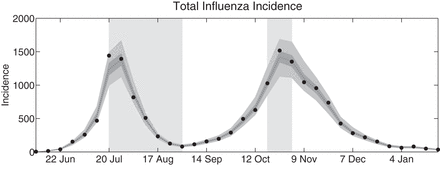
\includegraphics[width=\linewidth]{incidence.png}
    \vspace{1em}

    Time-varying factors: behaviour changes, preventive measures, seasonal effects, holidays
\end{frame}

\begin{frame}
\frametitle{Methodology: adding randomness}
Introduce randomness in the parameters (Bayesian) and model $\beta$ as a probability distribution. Assumption: population model, the random individual effects (biological factors, mode and frequency of travel) are aggregated in the data and hence captured in $\beta_t$.
$$\left\{\begin{array}{ll}\frac{dS_t}{d_t}=-\beta_t S_t \frac{I_t}{N}, \: \frac{dE_t}{d_t}=-\beta_t S_t \frac{I_t}{N} - kE_t, \: \frac{dI_t}{d_t}=kE_t-\gamma I_t, \: \frac{dR_t}{dt}=\gamma I_t \\ dx_t = \mu_x(x_t, \theta_x)dt+\sigma_x(x_t,\theta_x)dB_t, \: x_t=h(\beta_t)\end{array}\right.$$
Add diffusion process $x_t$ for $\beta_t$ which will solve the stochastic differential equations in our model.
$$\pi(x_{0:n}|y_{1:n}) \propto f(y_{1:n}|V_{0:n}, \theta_y) \times d\mathbb{P}_x \times \pi(\theta)$$
Sample the posterior of $x$ given the priors using a specific Markov Chain Monte Carlo (MCMC) type algorithm.
\end{frame}

\begin{frame}
    \frametitle{Motivation for Markov Chain Monte Carlo (MCMC)}
    \begin{itemize}
        \item Intractable integrals $\rightarrow$ approximate by sampling (Monte Carlo)
        \item No closed form of the density to sample from (by e.g. reverse integral transform) $\rightarrow$ use Markov chains
        \item A general name for algorithms based on this is Markov Chain Monte Carlo (MCMC)
    \end{itemize}
\end{frame}

\begin{frame}[fragile]
    \frametitle{Metropolis-Hastings (random walk Metropolis) example}
    \begin{lstlisting}
    mh <- function(target, starting, N) {
        x <- rep(0, N)
        x[1] <- starting
        for(i in 2:N) {
            last <- x[i-1]
            # Proposal from N(last, 1)
            p <- rnorm(1, mean=last, sd=1)
            # Compute acceptance probabilty
            accept <- target(p) / target(last)
            # Either with acceptance probability
            if(runif(1) < accept) {
                x[i] <- p
            } else {
                x[i] <- last
            }
        }
        return(x)
    }
    \end{lstlisting}
\end{frame}

\begin{frame}[plain]
    \begin{center}
    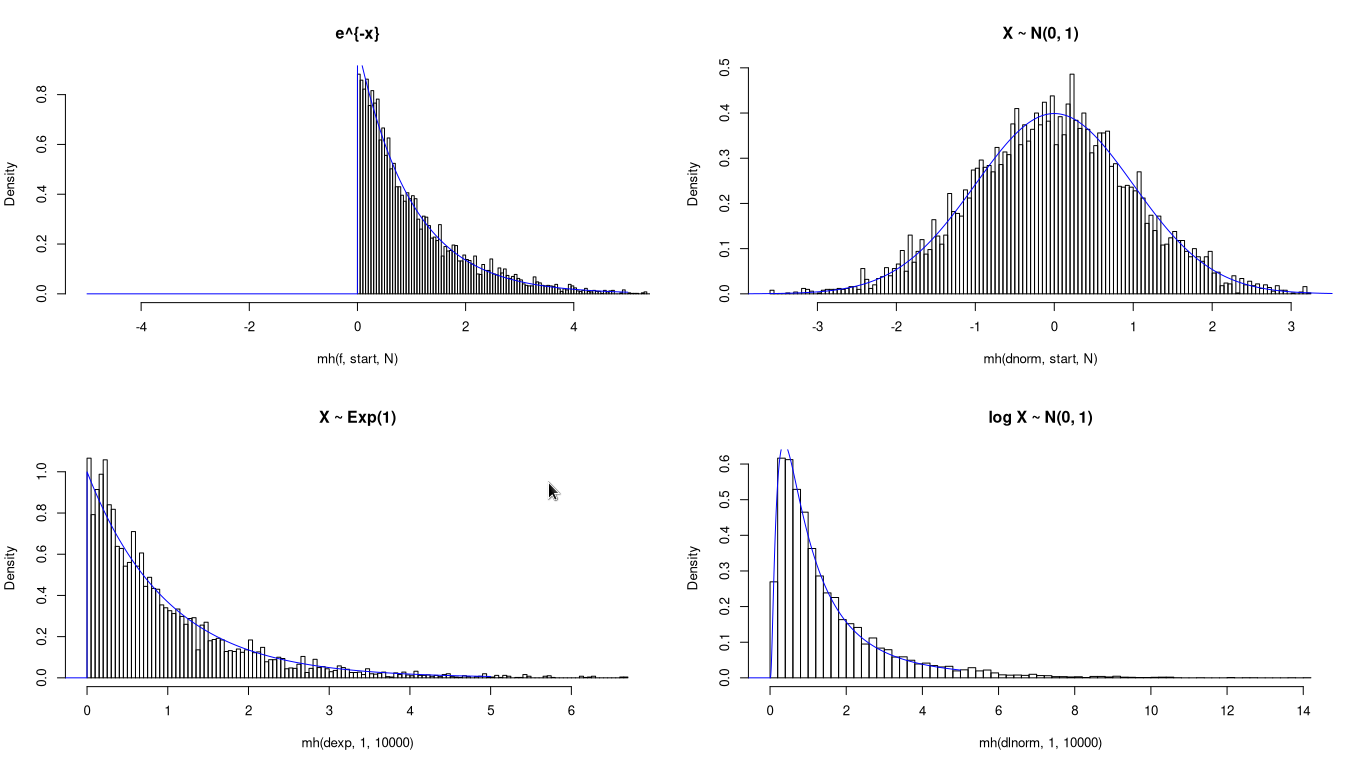
\includegraphics[width=\linewidth]{mh.png}
    \end{center}
\end{frame}

\begin{frame}
    \frametitle{Challenges of MCMC}
    \begin{itemize}
        \item Mixing -- relates to dependency of samples obtained with MCMC algorithm and how fast we can get them, can be assessed by Estimated Sample Size (ESS)
        \item Let $x_t=h(\beta_t)$ where $h$ is a positive-valued function, authors use natural log
        \item We want to obtain joint posterior density $p(x,\theta\:|\:y)$ -- this is a non-standard problem since
        \begin{itemize}
            \item The $x$ is high-dimensional (it’s the path of $\beta$)
            \item There is some dependence between $x$ and $\theta$
            \item In effect, classic methods are highly inefficient in mixing
        \end{itemize}
    \end{itemize}
\end{frame}

\begin{frame}
    \frametitle{Solution proposed by authors}
    \begin{itemize}
        \item Particle filters (PF) and Particle MCMC (PMCMC)
            \begin{itemize}
                \item PF gives us $p(x\:|\:y,\theta)$ and $p(y\:|\:\theta)$ (Doucet and Johansen, 2009)
                \item PMCMC gives us $p(x,\theta\:|\:y)$ (Andrieu et al., 2010)
            \end{itemize}
        \item There are still some issues with efficiency
        \item Adaptive Metropolis (Roberts and Rosenthal, 2009)
        \item Other methods such as Extended Kalman Filter (EKF) are considered but they require some assumptions which would contrain the generality of the proposed solution
    \end{itemize}
\end{frame}

\subsection{Results}

\begin{frame}
    \frametitle{Results: effect of school closures}
    \begin{columns}
    \begin{column}{0.5\textwidth}
    \begin{itemize}
        \small
        \item Black dots indicate estimates of observed incidence
        \item Grey rectangular areas indicate school breaks
        \item Dark and light area indicates the credible intervals
        \item Offline estimates of the effective contact rate
    \end{itemize}
    \end{column}
    \begin{column}{0.5\textwidth}
    \includegraphics[width=15em]{results.png}
    \end{column}
    \end{columns}
\end{frame}

\begin{frame}
    \frametitle{Results: effect of school closures}
    \begin{columns}
    \begin{column}{0.5\textwidth}
    \begin{itemize}
        \small
        \item Holidays periods have shown less total incidences.
        \item This could also mean that the epidemic had stopped because a critical population already had been infected, conferring that there is groups that have the immunity to stop the epidemic.
        \item The rise in influenza in the second grey area could contribute to the fact that schools were reopened and consequently effective contact rate increased them again.
    \end{itemize}
    \end{column}
    \begin{column}{0.5\textwidth}
    \includegraphics[width=15em]{results.png}
    \end{column}
    \end{columns}
\end{frame}

\begin{frame}
    \frametitle{Results: relationship between influenza cases and the real-time estimates}
    \begin{columns}
    \begin{column}{0.5\textwidth}
    \begin{itemize}
        \small
        \item Rise of H1N1 incidence fell throughout the school holidays and started rising again.
        \item An assumption could be made that decision-makers did not have access to the effective contact rate estimates data.
        \item From the data, it could be seen that the real-time estimates were still rising at the first grey area.
        \item Reopening schools while the effective contact rate was still rising contributed to another rise in total incidence.
    \end{itemize}
    \end{column}
    \begin{column}{0.5\textwidth}
    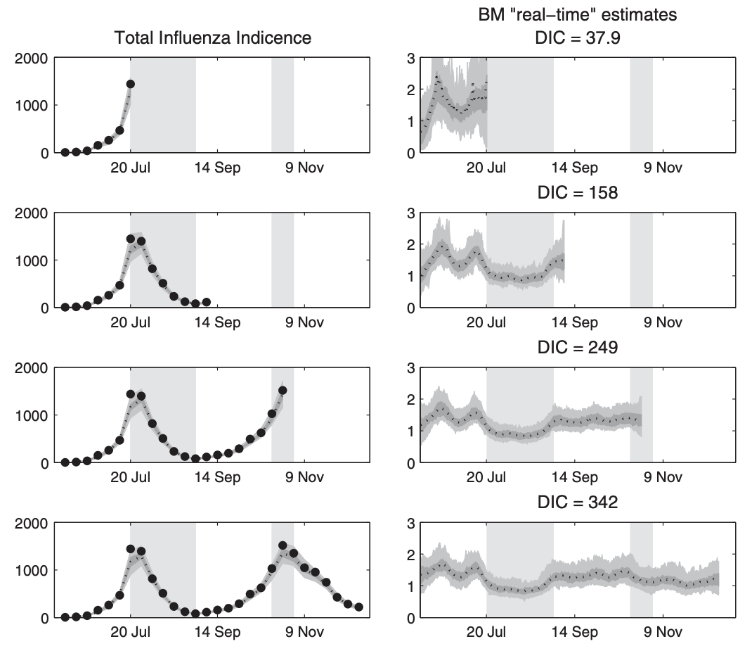
\includegraphics[width=15em]{time-varying.png}
    \end{column}
    \end{columns}
\end{frame}

\begin{frame}
    \frametitle{Results: relationship between influenza cases and the real-time estimates}
    \begin{columns}
    \begin{column}{0.5\textwidth}
    Some things to consider
    \begin{itemize}
        \item The effects of school holidays differ from children and adults
        \item We assumed here a homogeneous population.
        \item Will be more precise to consider a model with two age groups
    \end{itemize}
    \end{column}
    \begin{column}{0.5\textwidth}
    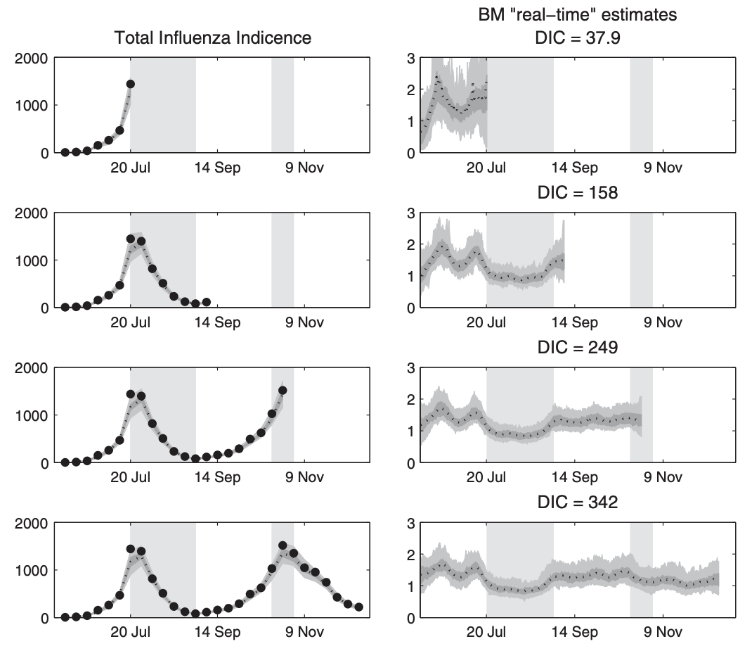
\includegraphics[width=15em]{time-varying.png}
    \end{column}
    \end{columns}
\end{frame}

\subsection{Evolution}

\begin{frame}
    \frametitle{Evolution of the subject}
    \begin{itemize}
        \item SSM: Inference for time series analysis with State Space Models. Dureau et al. 2013.
        \item Optimal control and the value of information for a stochastic epidemiological SIS-model. Grandits et al. 2019.
        \item Efficient real-time monitoring of an emerging influenza pandemic: how feasible? Birrell et al. 2019.
    \end{itemize}
\end{frame}

\section{Conclusion}
\subsection{Coronavirus}

\begin{frame}
    \frametitle{Conclusion: current coronavirus cases in China}
    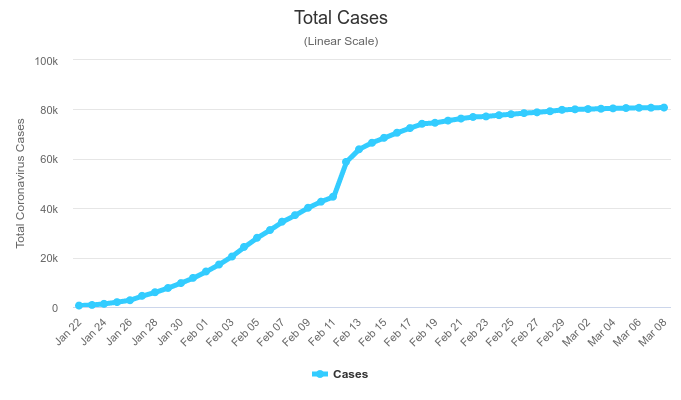
\includegraphics[width=\linewidth]{corona.png}
\end{frame}

\begin{frame}
    \frametitle{Conclusion: general remarks and questions}
    Bayesian Inference is a powerful tool, applicable to a vast range of problems. If you like the subject, consider taking ST308, a course on Bayesian Inference lectured by Dr Kalogeropoulos.
    \vspace{1em}

    We're now happy to take any questions. \\
    Feel free to message us at konstanty{@}kszk.eu
    \vspace{2em}
    \Large
    \begin{center}
    Thanks!
    \end{center}
\end{frame}

\end{document}

